\chapter{Apport}

\section{Introduction}

Il existe donc plusieurs possibilités pour appréhender l'informatique d'une façon divertissante, ludique et éducative. L'objectif de l'apport va être de proposer des idées dans ce sens et de également voir comment cela pourrait être implémenté. Est-ce que ces solutions sont implémentables en classe ? Quelles concepts sont abordés ? Est-ce que cela permet une réflexion personnelle de l'élève ? Comment amener l'élève à réfléchir d'un point de vue informatique au problème auquel il a été confronté ? Quel programme éducatif peut-on créer à partir de ces idées ?

Il me parait aussi très important que les solutions permettent l'interaction et qu'elles soient proche d'un environnement familier. En effet, cela permet d'améliorer l'implication de l'élève individuellement ou en groupe.

La possibilité d'accomplir des choses, de créer et de voir les résultats de sa création sont des sujets qui motivent l'élève, observations que nous avons notamment faites lors de l'état de l'art. Plus c'est visuel, plus l'élève est impliqué (en tout cas pour une initiation). Ainsi il me semble important de jouer sur ces facteurs. Si on arrive à faire quelque chose de visuel et dans un environnement familier on peut imaginer que cela peut amener à de meilleurs résultats.

L'apport n'a pas pour objectif de proposer des idées infaillibles et dont le résultat pédagogique est certain. Ce ne sont que des théories de ce qui pourrait être intéressant à mes yeux dans la pédagogie de concepts informatiques. On revient donc au point de départ avec la problématique du mémoire mais en ayant une idée de l'existant, cela va nous permettre de faire des remarques cohérentes sur les prises de décisions faites sur les solutions.

Le but est également de couvrir le maximum de concepts informatiques possibles, dans l'état de l'art nous avons pu voir que c'est surtout des concepts algorithmiques et de programmation qui étaient abordés. Ici, nous allons essayer, malgré le fait que l'on s'adresse à des enfants, d'aborder des notions variées et voir si elles sont transposables dans un programme d'éducation ou non. Même si elles ne sont pas complètes, nous proposerons au moins des ouvertures pour aller plus loin. Si certaines solutions hypothétiques peuvent se montrer non réalisables dans notre réalité (droits d'auteurs etc ...), on proposera alors une adaptation possible.

Concernant les critères de comparaisons nous utiliserons les mêmes que pour l'état de l'art, cependant nous ferons également en conclusion une comparaison de l'apport et de l'état de l'art concernant ces dits critères. Nous nous attarderons sur les différences entre les deux parties, pourquoi ces choix, avec un regard objectif sur l'apport et sa mise en oeuvre éventuelle dans la réalité.

\newpage

\section{Les solutions envisagées}

\subsection{Le Rubik's Cube, une énigme algorithmique}

Tout le monde connaît le Rubik's cube, ce casse-tête inventé dans les années 70. Casse tête géométrique en 3 dimensions, il est composé à l'extérieur de 26 cubes dont les faces peuvent se déplacer de droite à gauche (Voir figure). Si tout le monde connaît le rubik's cube, tout le monde ne sait pas le résoudre. On peut même être jaloux de ceux qui connaissent les systèmes de résolution du Rubik's Cube étant donné que l'on peut essayer de le résoudre pendant des heures sans y parvenir.

\begin{figure}[!htb]
  \centering
  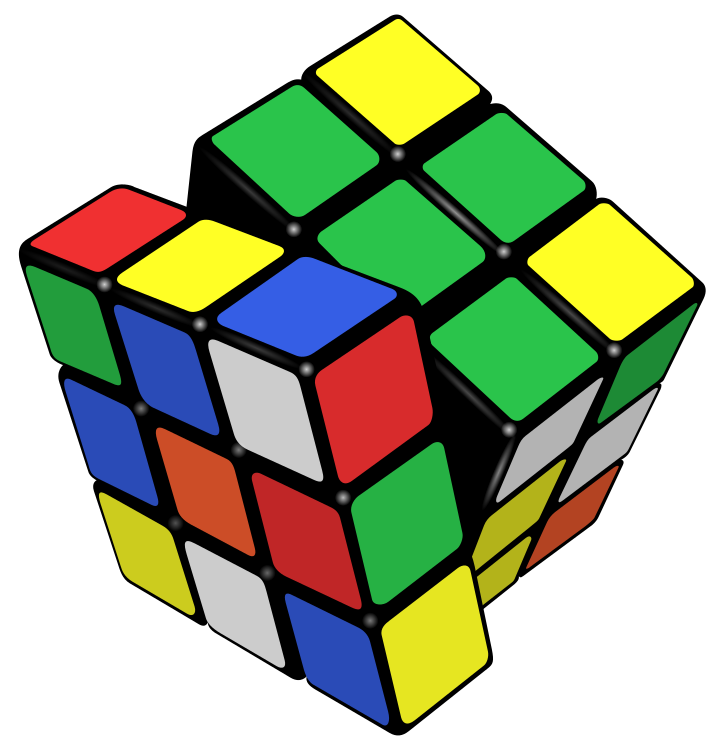
\includegraphics[width=30mm,scale=0.5]{images/rubiks-cube.png}
  \caption{Un Rubik's cube}
  \label{fig:boat1}
\end{figure}

Le Rubik's cube est donc composé de 26 cubes et 6 faces. Chaque cube a sa propriété : pièce centrale, pièce arête et pièce de bord. La pièce centrale est de une couleur, la pièce arête de deux couleurs et la pièce de bord de 3 couleurs. Les pièces centrales sont fixes, la blanche est toujours en face de la jaune, la rouge est toujours en face de la orange et la bleu est toujours en face de la verte. Les autres pièces tournent donc autour des centrales. Si nous modifions le cube en le mélangeant le but est donc de remettre en ordre les faces (c'est à dire une face, une couleur).

Maintenant, comment allons nous introduire les concepts d'algorithmes sur le Rubik's cube ? Avant toute chose, il faut définir les variables auxquelles nous allons exécuter des instructions. Tenons notre Rubik's cube de face et nous aurons donc une face avant, haut, droite et gauche. Ainsi à partir de là nous pouvons définir pour chaque face une variable. Par exemple h pour haut, d pour droite, g pour gauche, a pour avant, et b pour bas. Inutile de définir une variable pour la face arrière car nous n'en aurons pas l'utilité lors de la résolution du cube et l'utilisation d'algorithmes. Maintenant si on s'attarde aux mouvements possible du Rubik's cube, on peut affilier des instructions à ses variables. Quels sont les mouvements possibles si l'on a un rubik's cube de face ? On peut tourner 'a' vers la droite ou la gauche, 'd' en avant ou en arrière etc... Par conséquent, on peut définir a+ pour tourner la face avant dans le sens des aiguilles d'une montre et a- pour le sens contraire des aiguilles d'une montre. Par exemple, exécuter la commande 'tourner la face avant vers la droite' on l'a traduit alors par 'a+'. On peut ainsi définir un algorithme comme 'a+ b+ d-' sois trois instructions tourner la face avant à droite, la face bas en avant et la face de droite en avant (sens contraire aiguille d'une montre). Ce qu'il faut retenir c'est que '+' signifie qu'on est toujours dans le sens des aiguilles d'une montre pour une face. Il suffit alors de tourner le cube vers cette face pour être bien sur de son instruction (est-ce que je tourne bien dans le sens horaire?). Nous pouvons aussi introduire une instruction 'h2' comme 'tourner 2 fois la face du haut'.

Malgré le fait que l'on tourne le cube il faut toujours garder les même références c'est à dire que la face avant ne change pas lors du déroulement d'un algorithme et que, après une instruction, il faut toujours repartir de ce point de référence. Il faut donc par exemple se mettre en face de la face avant. Bien évidemment, ce que j'explique plus haut est bien plus clair lorsqu'on le fait avec un Rubik's cube entre les mains.

\newpage

Maintenant que nous avons expliqué brièvement comment on pouvait implémenter des variables et des algorithmes sur le Rubik's cube nous pouvons donner un exemple concret. Le Rubik's cube se résout en une multitude d'étape que l'on peut séparer facilement. La première étape de la résolution du Rubik's cube étant assez triviale il n'y a pas vraiment d'algorithme, il suffit d'avoir ce que l'on appelle la croix blanche (Voir figure). Si l'on est novice au Rubik's cube, cette étape sert notamment d'introduction aux mouvements du Rubik's cube et permet aussi une introduction à la visualisation dans l'espace, un autre point intéressant.

\begin{figure}[!htb]
  \centering
  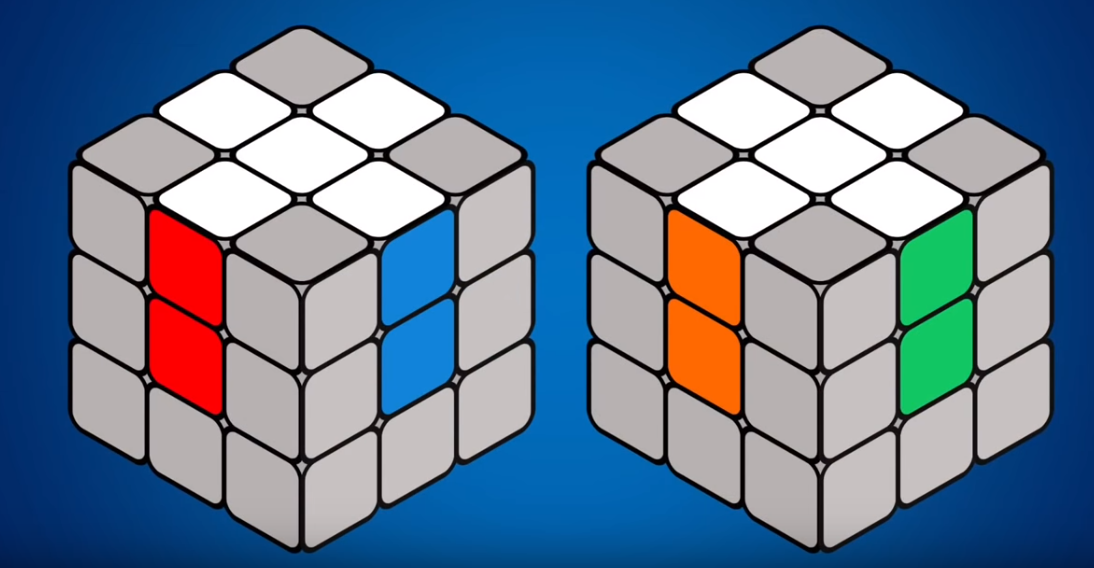
\includegraphics[width=60mm,scale=0.5]{images/rubiks-cube2.PNG}
  \caption{La croix blanche}
  \label{fig:boat1}
\end{figure}

Comme dit précédemment, comme cette étape est plutôt triviale il n'y pas vraiment d'algorithme, cependant il peut exister quelques cas particulier où l'on peut en appliquer. \cite{54}

Une fois qu'on a atteint cette étape,il faut remplir la face blanche. C'est un premier exemple d'utilisation d'algorithme dans le Rubik's cube. Comme on peut le voir dans la figure ci dessus, il reste alors 4 cubes contenant une face blanche. Nous allons les placer sous la position sur lesquels ils doivent être (donc sur la face du bas) et appliquer un algorithme. En partant donc de la référence croix sur la face du haut on applique : d- b- d+ b+. Bien sur dans ce cas la face dont la position doit être modifiée est en bas à droite par rapport à notre référence. Ce que l'on peut notamment observer sur cet algorithme c'est qu'il peut ne pas fonctionner du premier coup. En fait, dans ce cas il faut le boucler jusqu'à ce qu'il marche, pour expliquer cela dépend de l'orientation de départ de la face blanche sur le petit cube.

\begin{figure}[!htb]
  \centering
  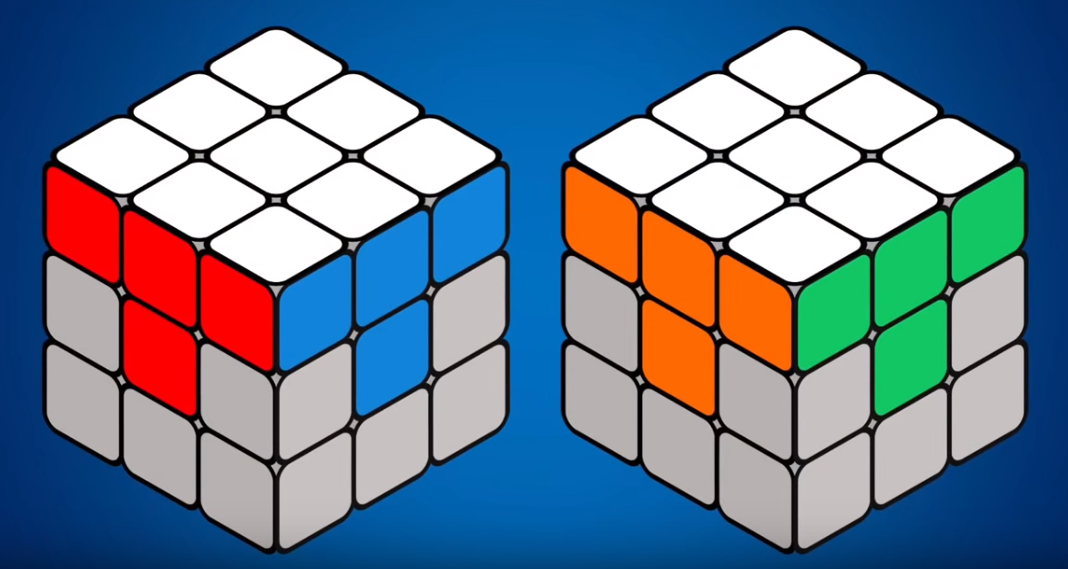
\includegraphics[width=60mm,scale=0.5]{images/rubiks-cube3.PNG}
  \caption{Face blanche complète}
  \label{fig:boat1}
\end{figure}

Ce qui est intéressant à partir de cette étape c'est que toutes les suivantes découlent d'autres algorithmes. Ces derniers sont relatifs aux cas particuliers sur lesquels on peut tomber. L'étape suivante consiste à faire ce qu'on appelle la deuxième couronne (voir annexe). Nous avons alors les deux premiers étages de la bonne couleur. Nous n'allons pas expliquer en détail la résolution du Rubik's cube ici, même si dans l'annexe sont définis tous les algorithmes pour tous les cas possibles et pour toutes les étapes. L'idée à travers cette partie était de montrer le lien entre le Rubik's cube et l'algorithmique.

\newpage

Quel lien peut-on faire avec l'éducation et pourquoi utiliser cet outil ? Une première chose importante à prendre en compte c'est que le Rubik's cube est connu et que le désir de le résoudre vient naturellement à nous. Même sans savoir le faire, en ayant un Rubik's cube dans les mains de par la popularité du casse-tête on tend forcément à faire des tentatives. Par conséquent, inculquer ce désir est déjà réussi et on part donc d'un bon début. Il est donc peu utile, même si on le refera quand même comme un rappel, d'expliquer les bases du Rubik's Cube. Dans tous les cas, cela sera simple chez les élèves. Étant donné sa popularité, il sera également gratifiant de savoir le résoudre ce qui rajoute une motivation. Au vu du nombre de personnes qui savent résoudre un Rubik's Cube, savoir le faire est une sorte de 'super pouvoir' qui peut le pousser à montrer ses capacités et le motiver encore plus.

D'un point de vue pédagogique, l'apprentissage de l'algorithme est présent. Les idées d'instructions, variable, suite d'instructions pour résoudre un problème se conceptualisent dans un environnement très concret. Par conséquent l'enfant peut comprendre 1) ce qu'est un algorithme, les instructions, les variables et 2) son utilité donc ici résoudre un problème qui peut être une étape ou le Rubik's Cube tout entier.

Si nous voulons apprendre le Rubik's Cube à des enfants il faut les accompagner en leurs faisant des cours. De plus, le concept de Rubik's Cube ne peut pas être appris à de très jeunes enfants (au moins fin primaire ou début collège). Pour les jeunes enfants, ils risquent de s'y perdre dans toutes les étapes qui existent dans la résolution du Rubik's Cube. Par conséquent si l'on doit faire un curriculum sur un cours sur le Rubik's Cube, il faudrait dans un premier temps enseigner les propriétés de ce dernier (les faces, les cubes, les couleurs, les règles, les orientations, les points de références, les types de cubes (arête, coin, centre)). Ensuite un cours sur l'explication des algorithmes avec le Rubik's cube puis des cours d'apprentissage de résolution de problème avec les algorithmes pour différentes étapes. Il peut aussi être intéressant d'expliquer pourquoi ces algorithmes fonctionnent. Il est également important de faire un cours récapitulatif sur les notions vues pour avoir une idée de la compréhension du problème et du sujet par les élèves. 

Cet apprentissage rejoint le concept d'apprentissage manuel vu notamment avec le CS Unplugged, on peut je pense réintégrer certains avantages connus de ce programme dans cette solution car encore une fois on apprend sans ordinateur. Également, en plus de l'informatique on peut rattacher à ce genre de cours à des problèmes de géométries étant donné qu'on doit souvent voir les problèmes dans l'espace pour les enfants. D'un point vue logistique, les rubik's cube sont très accessibles et facilement transposables dans une salle de classe.

Enfin, on peut faire une critique sur cette solution, en effet au vu des étapes différentes on peut penser que la complexité pour un enfant peut être rebutante, on peut s'y perdre facilement et l'apprentissage d'algorithmes pour les étapes peut être répétitif, même si de toute façon le but n'est pas de devenir un as un Rubik's Cube mais d'appréhender des notions d'informatique de façon ludique. 

On peut également se demander si la résolution du Rubik's Cube est accessible aux enfants. Sachant qu'il existe des enfants de 7 ans qui arrivent à le résoudre en moins de 30 secondes et à une main \cite{55} on peut supposer qu'avec un bon accompagnement cela est tout a fait atteignable pour des enfants de 10 à 14ans.

Bien évidemment il faut tester cette solution sur des classes d'enfants et voir si il y a des adaptations à faire notamment avec les problèmes de mémorisation qui peuvent survenir (en raison de toutes les étapes de résolution). Mais ce qu'on peut conclure c'est qu'il y a des avantages mathématiques (vision spatiale du problème) et informatiques (algorithme).

\newpage

\subsection{Minecraft et la redstone}

Minecraft est l'un des jeux incontournable de notre époque et il est aussi très populaire chez les enfants. C'est un jeu de type bac à sable où le joueur intervient dans un monde où il peut le modifier à sa guise. La construction y est complètement libre et permet de développer son esprit créatif. De plus, le jeu propose un mode de survie avec un système de jour et nuit où il faut se cacher des monstres la nuit. Pour cela le jeu propose un système d'artisanat qui permet au joueur d'évoluer dans ce monde virtuel. Tout est cube dans le jeu, chaque ressource est un cube et les constructions se font également cube par cube.

C'est un jeu extrêmement populaire, c'est même devenu récemment le jeu le plus vendu de tous les temps dépassant Tetris avec 176 millions d'exemplaires. \cite{56} Par conséquent il est une référence pour beaucoup d'enfants et cela en fait un environnement parfait pour l'apprentissage, en effet les enfants ont alors l'impression de jouer alors qu'ils apprennent. C'est notamment ce qu'à fait le site code.org qui propose des serious game pour les enfants. Parmis ces serious game existe un jeu inspiré de Minecraft. Ici c'est sous la forme d'un jeu drag-and-drop comme on a déjà vu précédemment dans l'état de l'art. \cite{57}

Ce qui nous intéresse dans Minecraft ce n'est pas le jeu à proprement parler mais une des fonctionnalité du jeu : la Redstone. C'est un élément du jeu qui sert de fil conducteur entre différents blocs. C'est à dire que l'on peut lier des blocs entre eux avec un fil conducteur (la redstone) et créer des systèmes logiques (la porte s'ouvre quand j'appuie sur le bouton).

La Redstone était initialement prévue pour augmenter la distance d'action d'un levier ou d'un bouton pour activer des objets mécaniques comme un piston, une porte etc. Aujourd'hui la redstone suit les logiques implémentées dans les circuits (comme les porte logique, OR, XOR, NOR, AND). Cette fonctionnalité permet donc de faire des circuits logique avec énormément de possibilités. Les plus acharnés on par exemple créé un calculateur de la suite de Fibonacci avec la Redstone. \cite{58} 

L'usage de la Redstone est simple même pour les nouveaux joueurs, dans un premier temps cela requiert juste de mettre un signal logique entre un actionneur et un déclencheur (voir la figure ci dessous). Le signal rouge visible sur le sol a une limite de 16 blocs qu'il faudra alors allonger avec un répéteur, un objet du jeu qui a de multiple propriétés dans les circuits (retardateur, alimentation, mémorisation).

\begin{figure}[!htb]
  \centering
  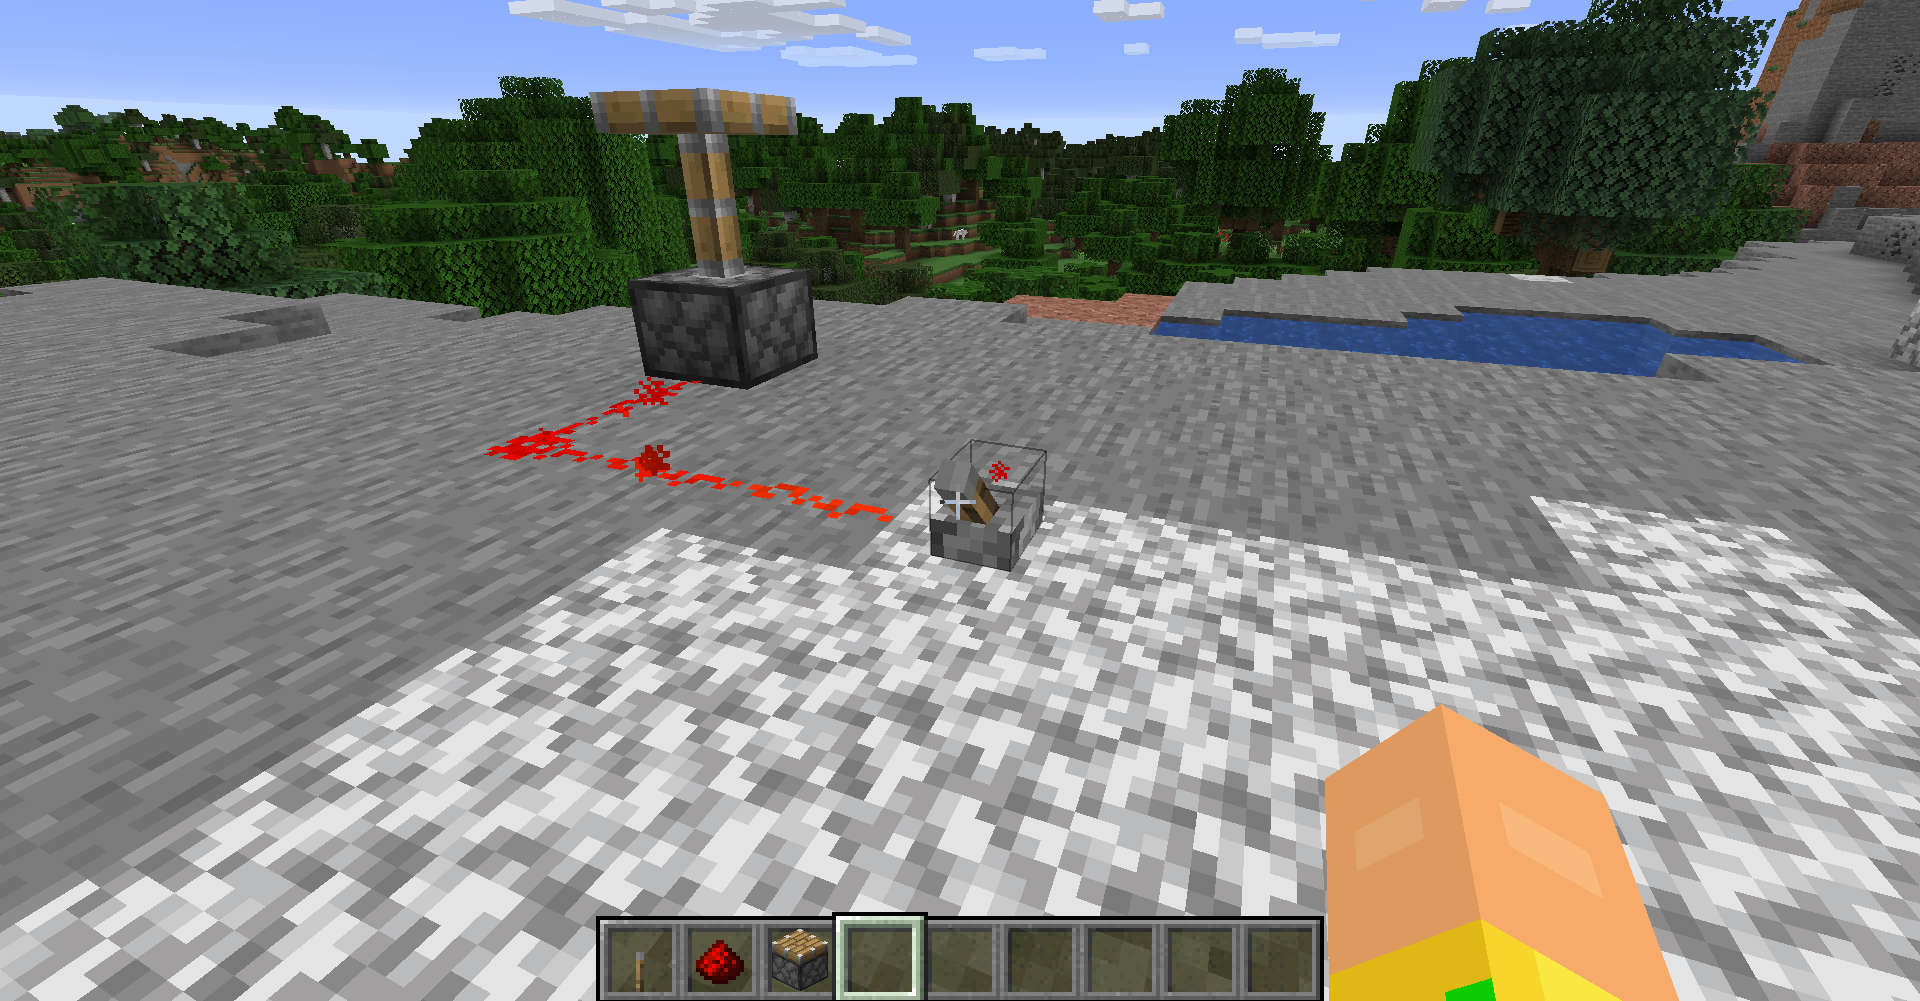
\includegraphics[width=75mm,scale=0.5]{images/minecraft.png}
  \caption{Activer un piston avec de la redstone et un levier}
  \label{fig:boat1}
\end{figure}

Partant de ce simple statut, les possibilités sont très grandes car on peut faire des systèmes autonomes utilisant les portes logiques, table de vérités etc. Il existe en fait énormément de blocs dans le jeu liés à la redstone qui permettent ces grandes possibilités. \cite{59} Ici, nous ne ferons pas d'explication détaillée sur la redstone et nous n'allons pas apprendre comment faire une calculatrice sur Minecraft (même si c'est possible). Nous allons plutôt voir comment implémenter les portes logiques.

\newpage

Avant d'expliquer les portes logique il faut introduire le système de torche de redstone, visible dans la citation précédente. Ces torches servent à faire passer le courant. Elles sont, par défaut, allumées, pour en éteindre une, il faut passer du courant dedans et ce courant passe par le bloc qui sert de socle à la torche. On peut voir ce fonctionnement dans les figures ci dessous.

\begin{figure}[!htb]
  \centering
  \begin{minipage}[b]{0.45\textwidth}
    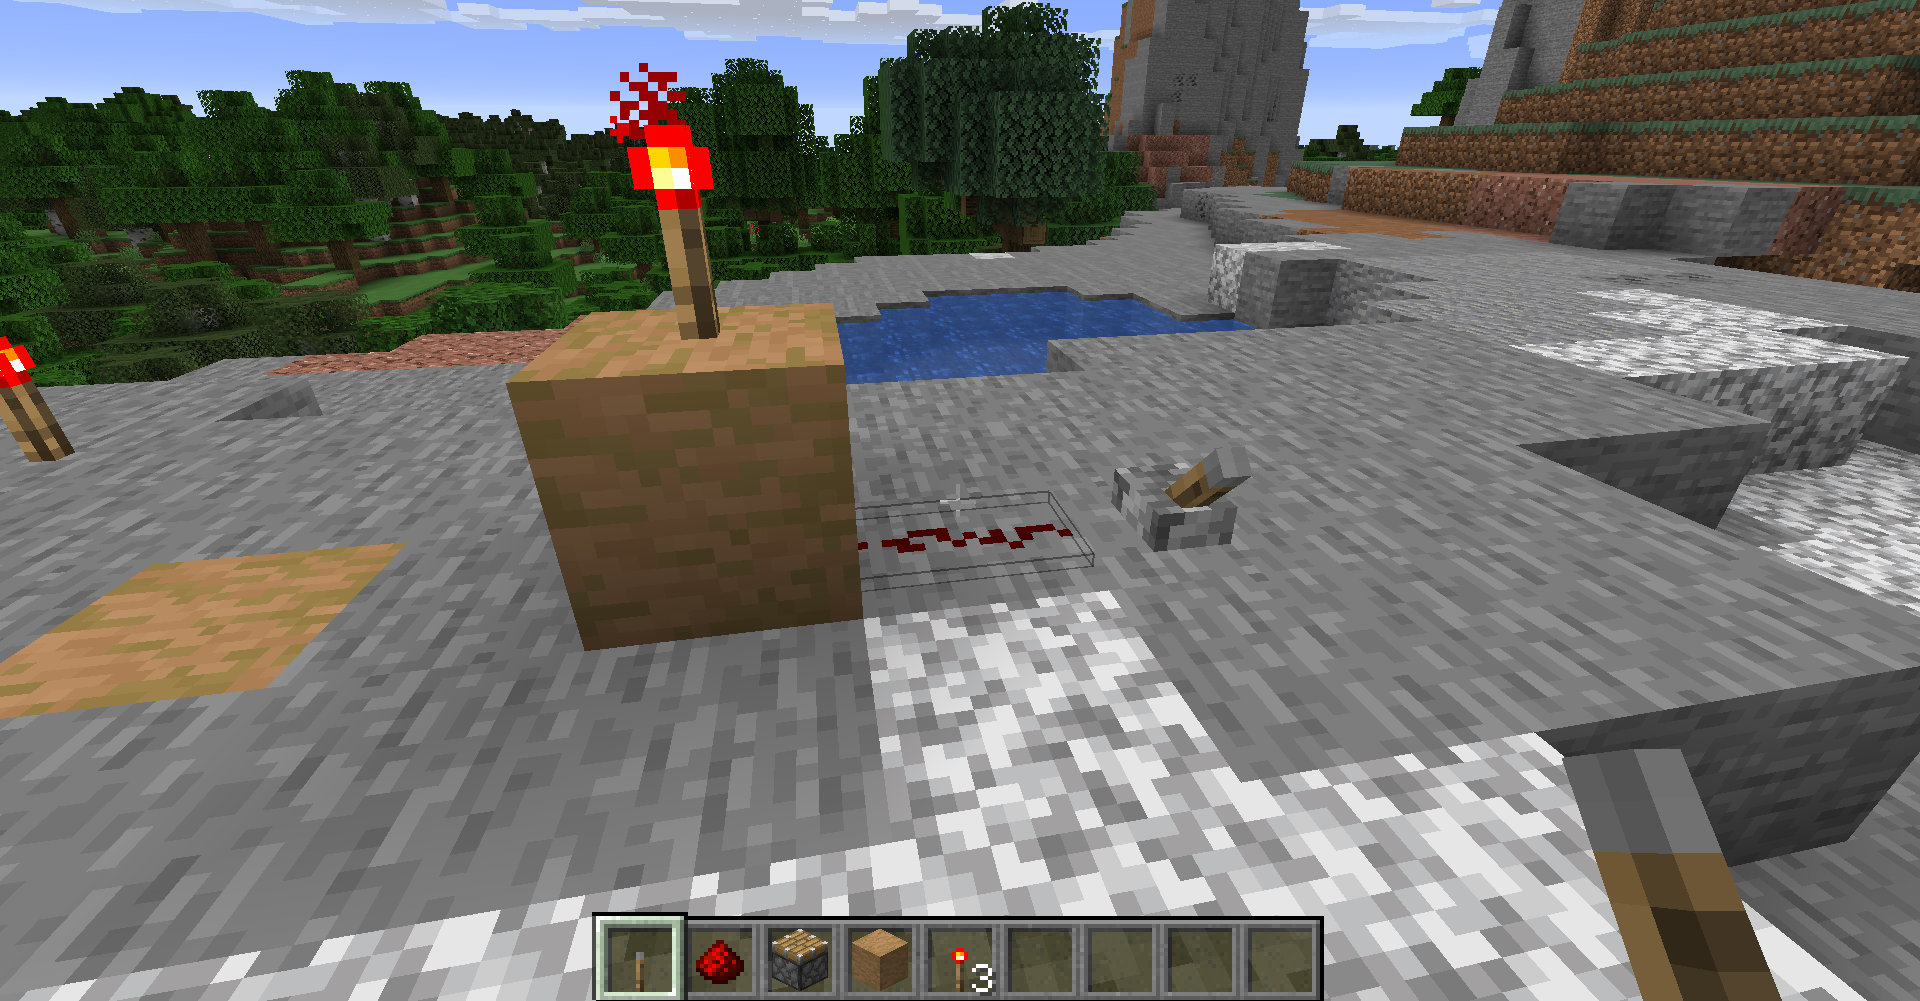
\includegraphics[width=\textwidth]{images/minecraft2.png}
    \caption{Levier éteint, la torche est allumée (par défaut elle est)}
  \end{minipage}
  \hfill
  \begin{minipage}[b]{0.45\textwidth}
    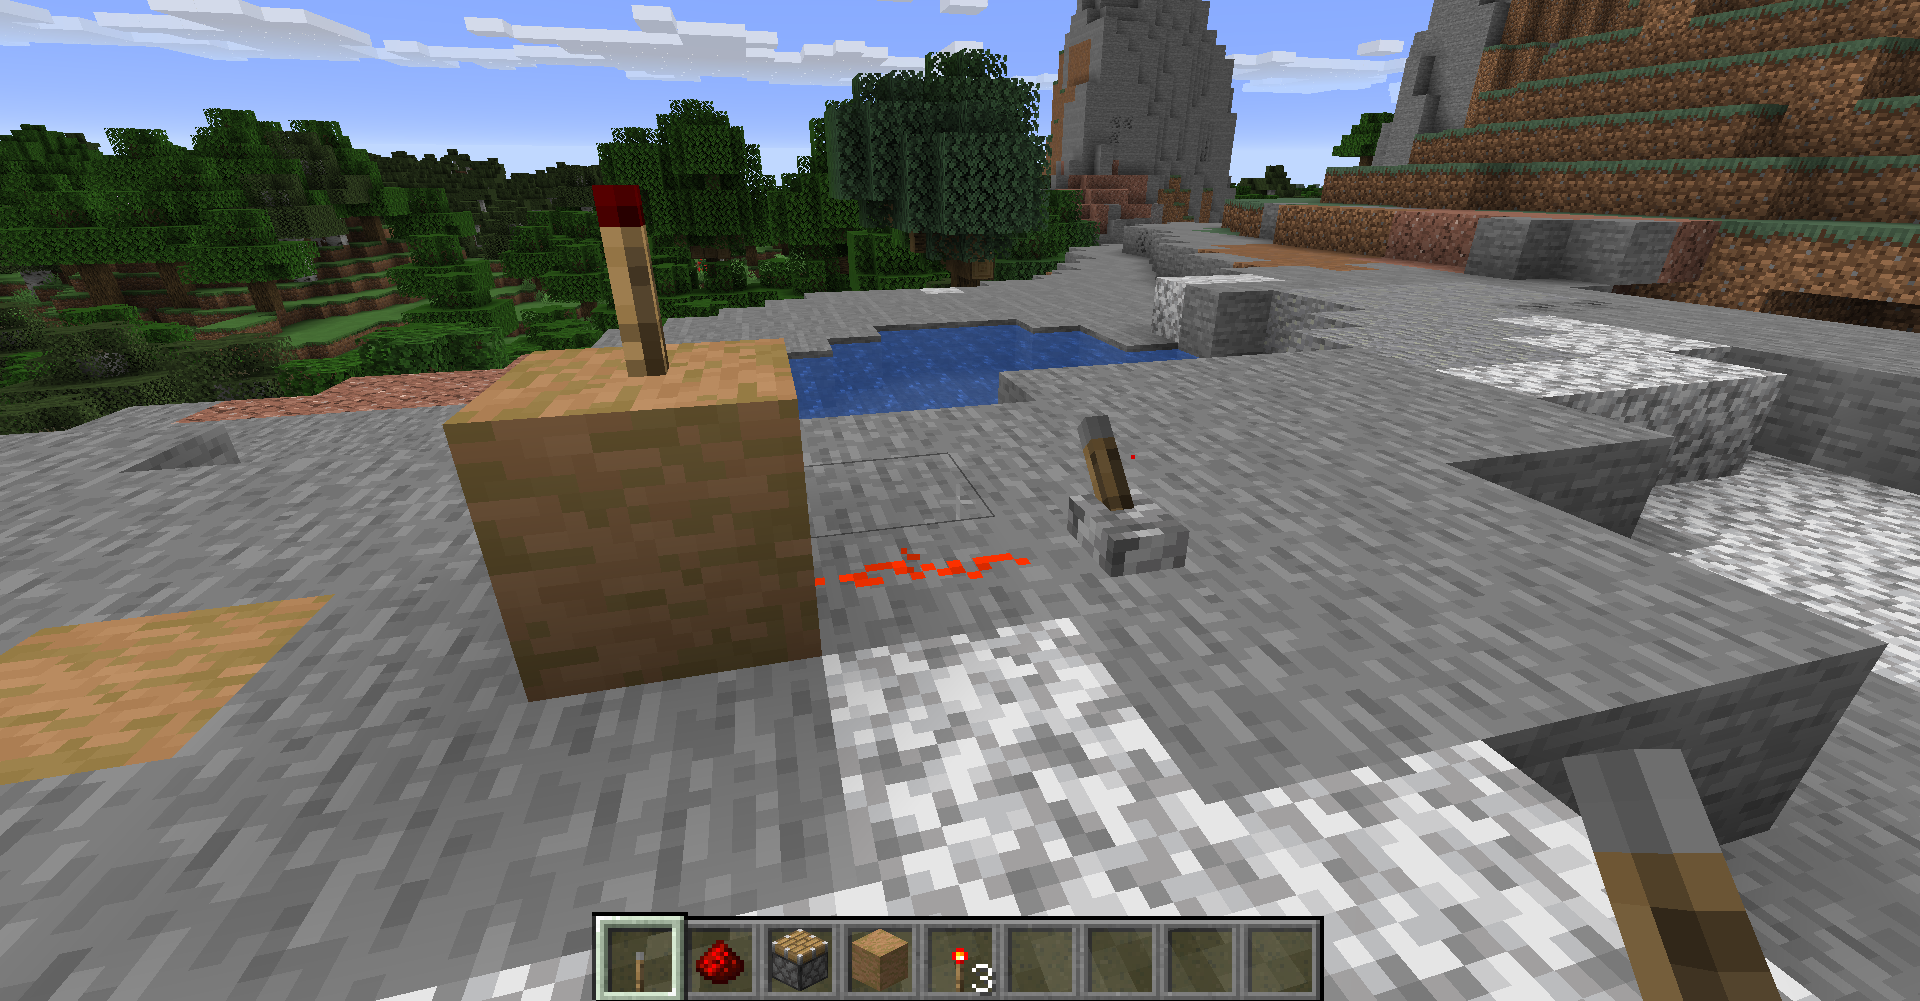
\includegraphics[width=\textwidth]{images/minecraft3.png}
    \caption{Levier allumé, on passe le courant au bloc socle, la torche s'éteint}
  \end{minipage}
\end{figure}

Maintenant que ce système est compris, on peut implémenter avec la redstone l'opérateur booléen AND. C'est à dire qu'on va avoir deux leviers et c'est seulement quand les deux sont allumés qu'un piston va s'activer. Ce système est visible avec la figure ci dessous.

\begin{figure}[!htb]
  \centering
  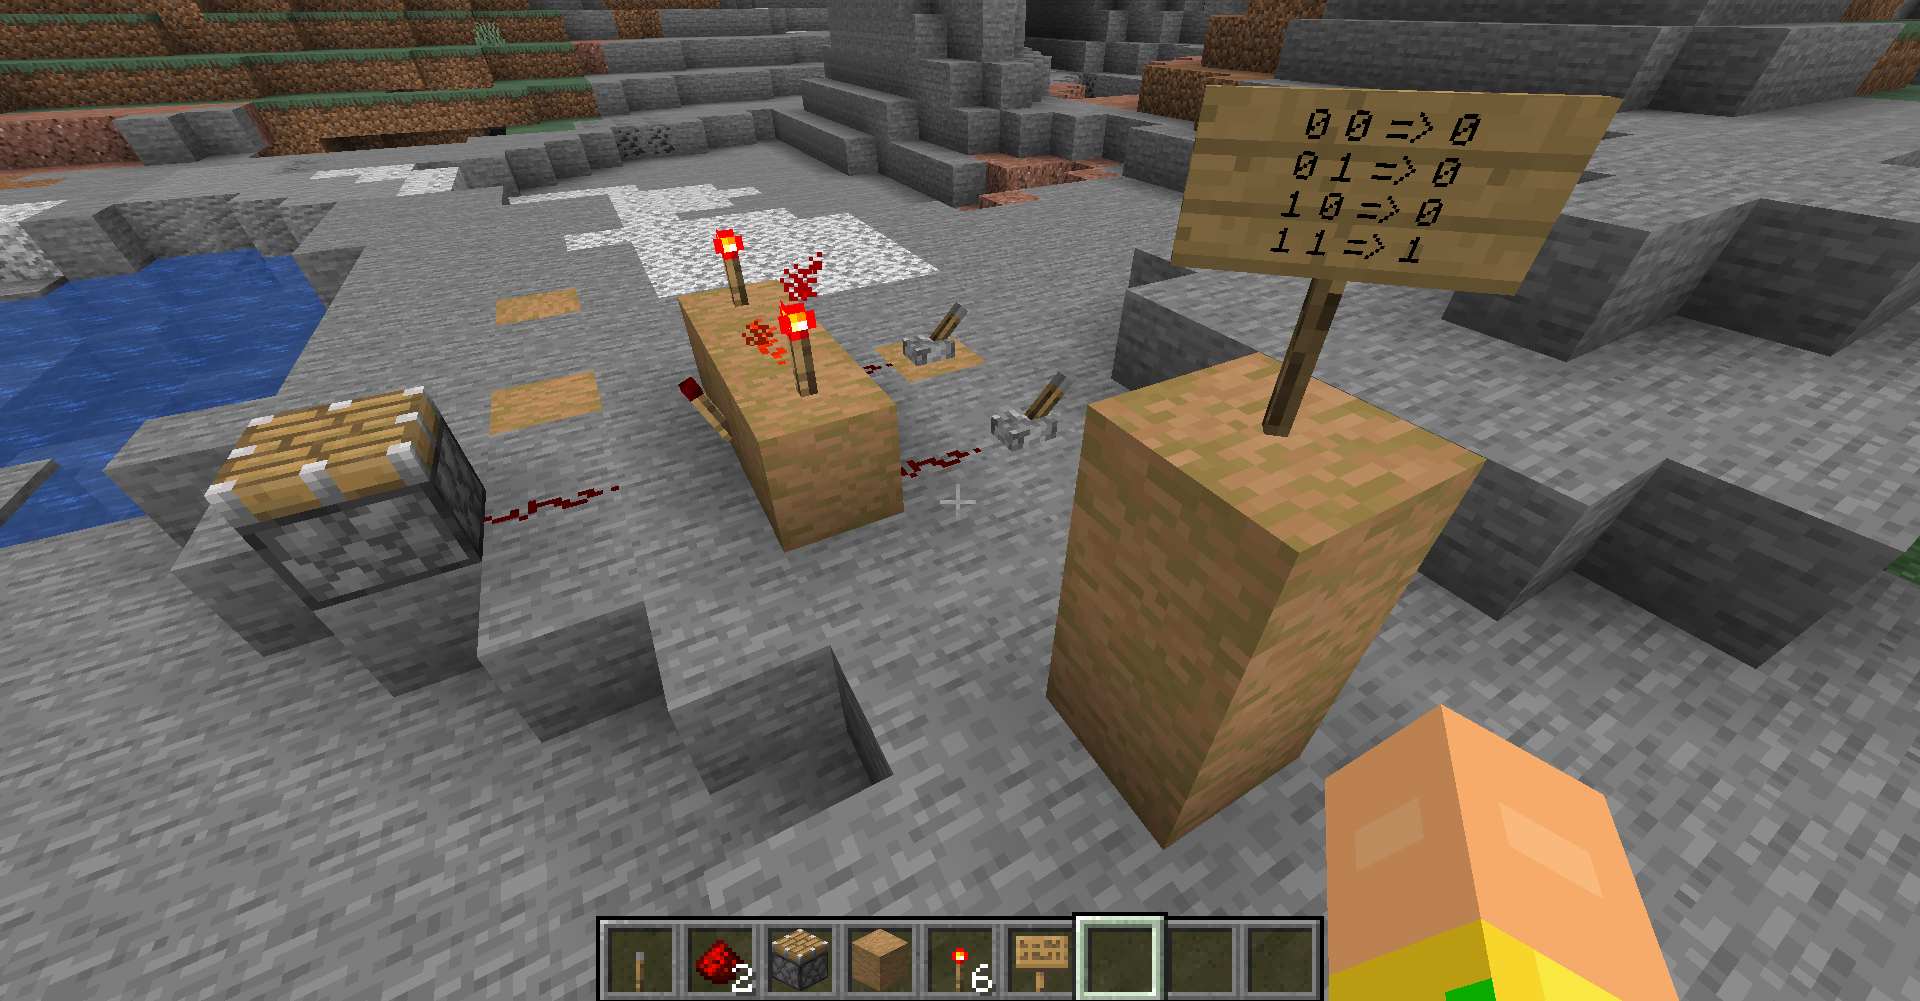
\includegraphics[width=90mm,scale=0.5]{images/minecraft4.png}
  \caption{Implémentation de l'opérateur booléen AND, le panneau résume les états possibles des leviers}
  \label{fig:boat1}
\end{figure}

Dans l'image, nous avons le premier état écrit sur le panneau de la capture d'écran sois 0 0. En effet comme on peut le voir, aucun courant passe dans les signaux par terre (à droite), si on active un levier on sera dans le cas 0 1 ou 1 0 et par conséquent le piston ne va toujours pas s'activer. En effet il y aura toujours une des deux torches allumées sur les blocs ce qui fera que le courant sur le bloc centrale sera toujours actif. Dans le cas où l'on active les deux leviers, les deux torches sur les blocs vont s'éteindre, le courant qui passe entre ces deux blocs va s'éteindre également et étant donné qu'il n'y aura plus de courant qui passera dans le bloc socle central, la troisième torche s'allumera ce qui fera passer le courant dans le circuit à gauche et qui activera le piston. Ce système est bien plus compréhensible avec le jeu en face de nous car dans ce cas on peut interagir, et mieux comprendre les différentes propriétés des blocs. On peut préciser que dans notre exemple nous avons deux entrées mais il est possible de faire des systèmes à 4, 8 ou 16 entrées.

On peut également parler de l'opérateur logique OR, encore plus simple d'implémentation, si nous prenons un cas à deux entrées comme l'exemple précédent, il suffit alors d'activer seulement un des deux leviers pour activer le piston. Cette exemple est visible dans la figure ci dessous.

\newpage

\begin{figure}[!htb]
  \centering
  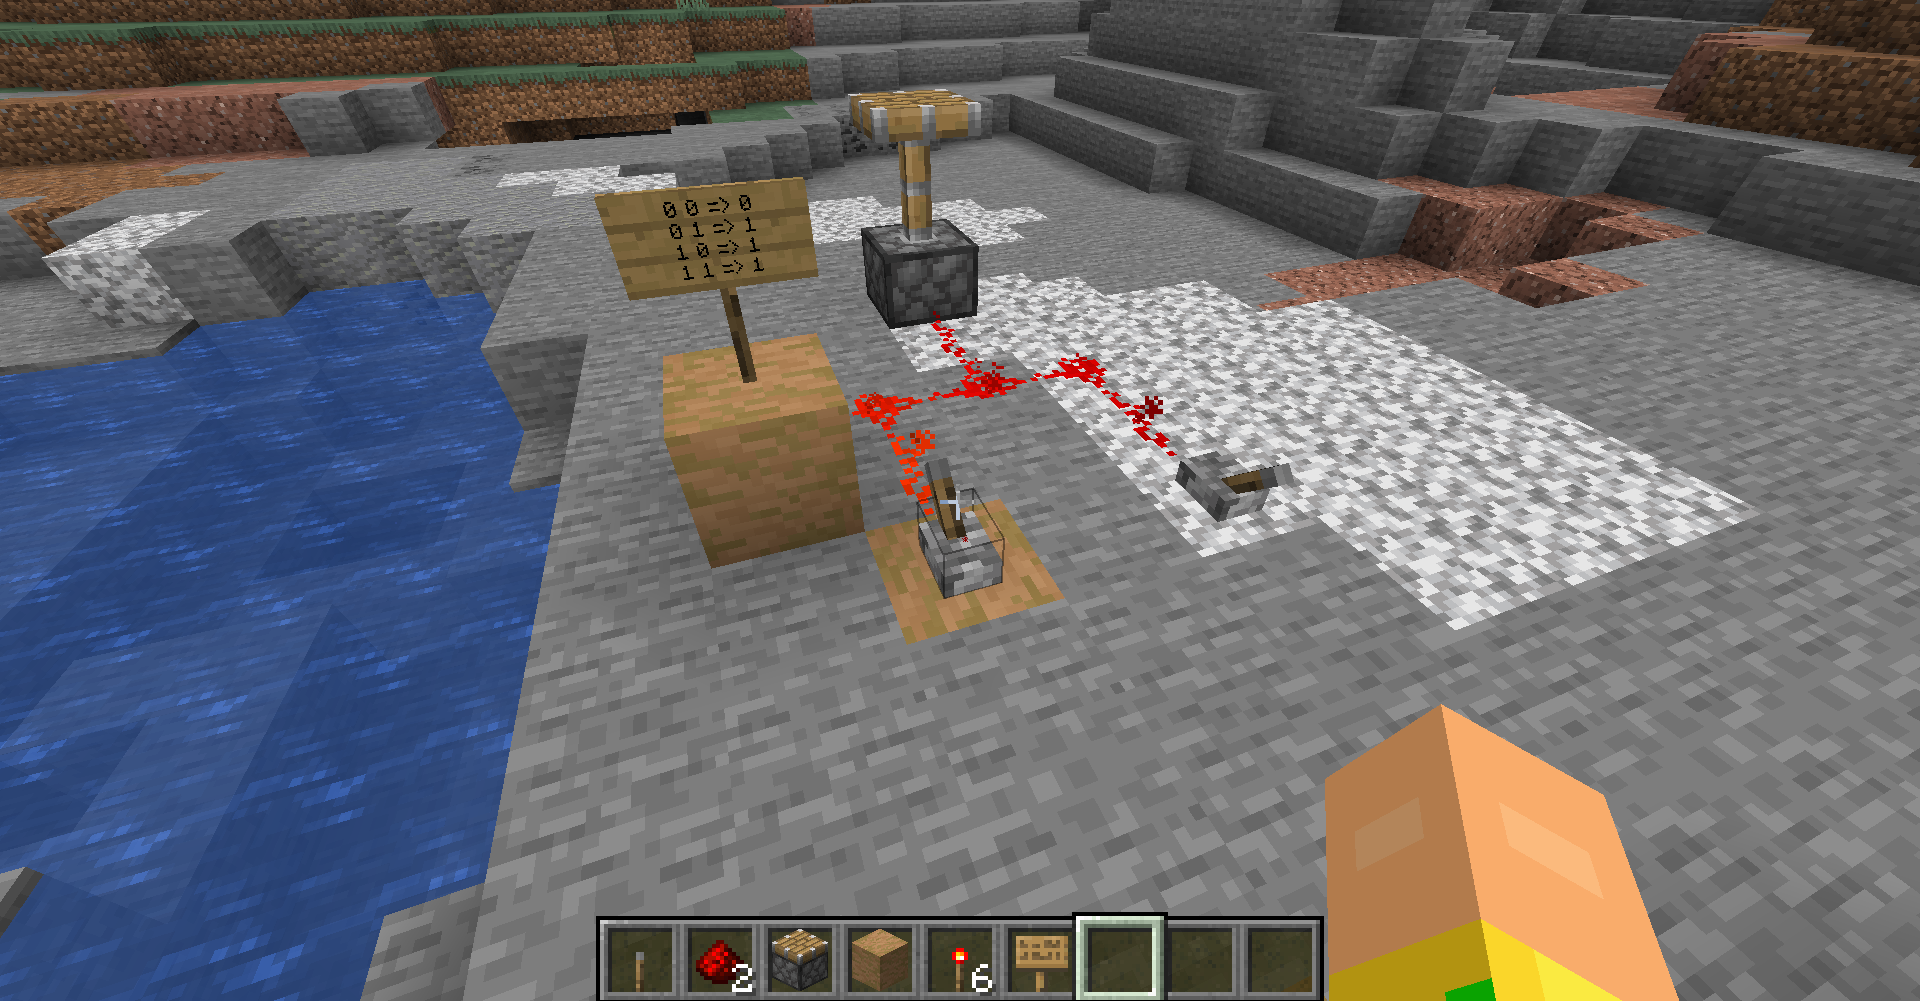
\includegraphics[width=100mm,scale=0.5]{images/minecraft5.png}
  \caption{Opérateur OR, dans le cas 1 0}
  \label{fig:boat1}
\end{figure}

Dans cette figure on observe que l'on a activé le levier de gauche et non celui de droite et cela active quand même le piston. Un seul levier activé fait passer le courant ici. Nous pouvons implémenter d'autres opérateurs logiques comme le NAND, NOR, XOR, XNOR mais nous n'allons pas ici tous les définir. Certains autres exemples sont cependant disponibles en annexe.

Les opérateurs booléens ne sont pas les seules possibilités avec Minecraft, ici nous abordons vraiment les bases de ce que l'on peut faire avec la Restone. Il existe aussi la possibilité de faire des mises en mémoire tampon et des systèmes complexes (comme par exemple certains joueurs qui ont fait une calculette avec la Redstone \cite{60}) Nous n'allons pas tout aborder ici mais cela montre que les possibilités de problèmes logiques et algorithmiques que nous pouvons créer sont très grands. Étant donné que Minecraft est un jeu de construction composé de blocs qui fait que tout le terrain est modifiable les limites sont presque infinies.

Quel rapport peut-on faire entre ces faits et l'éducation ? Comme dit précédemment Minecraft est un jeu très populaire et par conséquent le fait que les élèves soient impliqués dans des exercices en rapport avec Minecraft augmente les chances d'attention de ces derniers. Ensuite, les exercices avec la Redstone permettent à l'enfant d'entrevoir les notions d'entrées sorties, de binaire, comment marche un circuit électronique, les opérateurs booléens et par conséquent des notions algorithmiques.

Si l'on veut transposer Minecraft dans un programme éducatif on pourrait par exemple réfléchir à des cours d'initiation à la redstone et à son fonctionnement, d'initiation aux opérateurs booléens et d'exercices pratiques impliquant la redstone (imaginons par exemple, faire un système de mots de passe à 5 leviers pour ouvrir la porte de sa maison). Cependant, il ne faut pas oublier que Minecraft est un jeu vidéo et que par conséquent l'élève risque de tenter de vraiment jouer au jeu plutôt que de se focaliser sur la redstone. Pour cela, il faudrait mettre en place une structure restrictive qui ne permet pas d'accéder aux fonctionnalités du jeu (survie, exploration etc...) mais qui se focalise sur la redstone et sur la créativité. Imaginons par exemple une carte vierge où l'on a les blocs strictement nécessaire à l'exercice. 

Enfin, le jeu est payant ( \EUR{23,95}) et par conséquent le mettre en place dans les écoles impliquerait d'acheter des licences ce qui peut être parfois rébarbatif quand on propose une solution encore jamais explorée et dont les résultats pédagogiques sont incertains.

\newpage

\subsection{World Of Warcraft pour apprendre le SQL ?}

Comme Minecraft, World Of Warcraft est un jeu très populaire. Cependant, contrairement à Minecraft il est très complexe. C'est un jeu en ligne multijoueur qui se déroule dans un univers fantastique. Deux factions se combattent et chaque faction possède ses différentes races de personnages. Un personnage dans le jeu appartient à une classe (mage, guerrier, prêtre ...). Chaque classe à des sorts, compétences, spécialisations. Le personnage progresse dans un monde virtuel où il navigue entre différentes zones du jeu, rencontre d'autres personnages (joueur et non joueur) et participe à des quêtes, ramasse des objets etc... Cette complexité dans l'univers de World Of Warcraft fait que toutes ces données doivent être rangées dans une base de données et que des liens doivent être faits entre les différentes tables de la base.

Lorsque j'ai personnellement voulu essayer de faire un serveur World Of Warcraft dans sa version Vanilla (donc sans extension), j'ai utilisé un système qui s'appelle MaNGOS. \cite{61} \cite{62} Par exemple pour World Of Warcraft Vanilla, il partage un serveur, une base de données et les scripts pour le jeu. Une fois toute l'installation faite, nous avons donc accès à cette base de données qu'il faut de toute façon obligatoirement modifier pour mettre en place le serveur.

MaNGOS propose en faite une base de données calquée sur le modèle de World Of Warcraft (donc recréée) avec sa documentation complète. \cite{63} Il y a plus précisément deux bases de données "mangos" pour le jeu et "realmd" pour tout ce qui est compte et serveur. Faisons par exemple un 'SHOW TABLES' sur realmd on obtient le tableau suivant.

\begin{table}[!htb]
\centering
\begin{tabular}{|l|}
\hline
Tables\_in\_realmd    \\ \hline
account               \\
account\_access       \\
account\_banned       \\
antispam\_blacklist   \\
antispam\_detected    \\
antispam\_replacement \\
antispam\_unicode     \\
ip2nation             \\
ip2nationcountries    \\
ip\_banned            \\
migrations            \\
realmcharacters       \\
realmlist             \\
uptime                \\ \hline
\end{tabular}
\end{table}

Si par exemple nous faisons un 'SELECT * FROM account' nous aurons la liste des comptes suivant ce schéma \cite{64} et si nous faisons 'SELECT * FROM realmlist' nous aurons la liste des serveurs suivant ce schéma. \cite{65}

Ce qui est maintenant intéressant c'est qu'une action sur ces tables entraînera alors le fait que l'on peut par exemple se connecter avec un nouveau compte sur le jeu (si l'on a fait un INSERT INTO d'un n-uplet) ou qu'on ne peut par exemple plus se connecter sur un compte (si l'on a fait un DELETE sur une ligne). Il en va de même pour les serveurs.

Pour l'autre base de données, en plus de pouvoir effectuer des actions similaires (retrait de sort, ajout d'un personnage non joueur...). On utilise en plus le système de clé primaire pour faire le lien entre les tables. Imaginons que nous voulons créer une creature suivant ce modèle :

\begin{lstlisting}[frame=single]
(guid, id, map, modelid, equipment_id, position_x, position_y, 
position_z, curhealth, curmana, DeathState, MovementType)
\end{lstlisting}

Il faut alors faire référence à un modelid qui suit ce modèle 
\begin{lstlisting}[frame=single]
(modelid, bounding_radius, combat_reach, gender)
\end{lstlisting}

Ainsi après avoir inséré notre créature avec ses paramètres et sa position il sera directement visible dans le jeu. C'est ici que c'est ludique, car nos actions dans la base de données font que le jeu est modifié et c'est visible directement. Il est alors amusant de voir toutes les possibilités que l'on a en changeant cette base de données (modifier la taille de certains personnage, changer les positions de départ des joueurs après avoir créé un personnage). Il est aussi très intéressant de voir comment marche une base de données dans un cas concret et les liens entre les classes. Si nous voulons voir ça d'un point de vue éducatif, il faudrait alors apprendre les structures d'une base de données et apprendre dans un premier temps comment on navigue dedans. Ensuite on pourra apprendre les commandes de base du SQL (SELECT, UPDATE, DELETE ...) et voir leurs effets directement dans le jeu.

Cependant, travailler avec la base de données MaNGOS est complètement inconcevable dans un cadre éducatif et ça pour plusieurs raisons. Dans un premier temps la base de données est très complexe et pas forcément évidente, certaines tables utilisent trop de données souvent incompréhensibles pour quelqu'un de non initié. Les noms de tables ne sont pas familiers, les paramètres sont incompréhensibles etc... Ensuite, aussi parce que World Of Warcraft appartient à une entreprise. Il est complètement illégal d'utiliser son logiciel de cette façon et cette base de données (MaNGOS) aussi. Le jeu n'est pas du tout adapté pour ce genre d'utilisation vu qu'il est utilisé pour le jeu en ligne. Enfin, World Of Warcraft est un jeu déconseillé pour les enfants.

Le point essentiel de MaNGOS et de sa base de données est que l'utilisation et la modification de cette dernière est divertissante tant on voit l'impact qu'elle a sur le jeu. On a alors envie de découvrir par nous même cette base et y appliquer des modifications pour créer toutes sortes de scènes, parfois surréalistes, parfois pour tricher dans le jeu tout simplement. C'est cet effet que ça a eu notamment sur moi qui me semble important pour le point de vue pédagogique. Comme pour Minecraft, on a l'impression de jouer en apprenant.

MaNGOS n'est au final qu'un prétexte. C'est pour faire comprendre qu'en réalisant un environnement fait pour l'apprentissage utilisant le SQL, on pourrait créer quelque chose de ludique autour de cette technologie. Imaginons maintenant une base de données semblable à MaNGOS mais sans sa complexité. C'est à dire que l'on garderait un univers fantastique comme World Of Warcraft (Race, classe, spécialité etc...) ou tout serait stocké dans une base de données. Ensuite une modification de cette base entraînerait une modification dans un univers virtuel semblable à World Of Warcraft. Par conséquent avec un tel système, on serait capable d'impliquer l'enfant dans une base de données et son fonctionnement grâce à l'environnement proposé. On pourrait alors lui apprendre à naviguer dans la base avec des noms de tables parlant (creature, personnage, sort, quête). Et lier ces tables entres elles (un n-uplet de quête lié à l'id d'un personnage) et pouvoir faire des modifications facilement dans cette dernière.

Si on veut créer un dispositif d'enseignement autour de cette idée, il faudrait dans un premier temps créer le logiciel et ensuite réfléchir aux exercices à faire dessus. L'important étant d'aborder des points comme : comment fonctionne les bases de données, comment naviguer dans une base de données, quels sont les commandes de bases d'une base de données et quels sont les effets de ces commandes.

\newpage

\subsection{Le cas Raspberry Pi}

Le Raspberry Pi est un micro-ordinateur au prix de vente faible (environ \EUR{25} ). Cela permet une bonne distribution du produit. Si l'on prend du recul on peut même dire que cela peut être une solution pour des pays en voie de développement qui ne peuvent pas avoir un accès facile aux ordinateurs dans un cadre éducatif. Raspebrry Pi est distribué en général sous Linux, ce système d'exploitation souvent mystérieux pour beaucoup de personnes. Ce qu'il faut savoir sur cet ordinateur c'est qu'il a pour but d'encourager ses utilisateurs à l'apprentissage de la programmation informatique. C'est ce qui est directement visible sur le site officiel. \cite{66}

Malgré cela, notamment en France, il n'existe pas vraiment de programme d'éducation comprenant le Raspberry Pi. Pourtant, étant sous Linux, il permettrait aux enfants de découvrir cet environnement et notamment les commandes Unix (par exemple se déplacer dans les fichiers de l'ordinateur sans passer par un explorateur de fichier graphique). Il serait notamment intéressant d'apprendre d'autres commandes Unix dans un environnement ludique. Imaginons par exemple créer un serveur Minecraft sur une raspberry en passant par la console. \cite{67} Ensuite, on pourrait expliquer comment modifier les fichiers de configuration depuis la console également (à la création d'un serveur Minecraft nous sommes obligés de modifier un fichier qui stipule qu'on accepte le terme EULA, soit passer une variable dans un fichier texte à 'true'). Il est aussi possible de faire un lien pédagogique avec des notions de réseau (Pourquoi je peux me connecter sur mon serveur Minecraft en 127.0.0.1 ? Qu'est-ce que le port 25565 sur mon serveur ? pourquoi les autres joueurs peuvent rejoindre mon serveur ? Qui est le client et qui est le serveur ?)

Rien qu'avec Minecraft, qui nous permet plus facilement de communiquer avec les enfants, il y a beaucoup de possibilités envisageables avec le Raspberry. Surtout que comme dit précédemment, ce dernier a une volonté à la base pédagogique, comme ce qui est énoncé sur le site : "\textit{A small and affordable computer that you can use to learn programming}" . C'est notamment ce qu'on observe directement en se baladant dans la barre de tâche.

\begin{figure}[!htb]
  \centering
  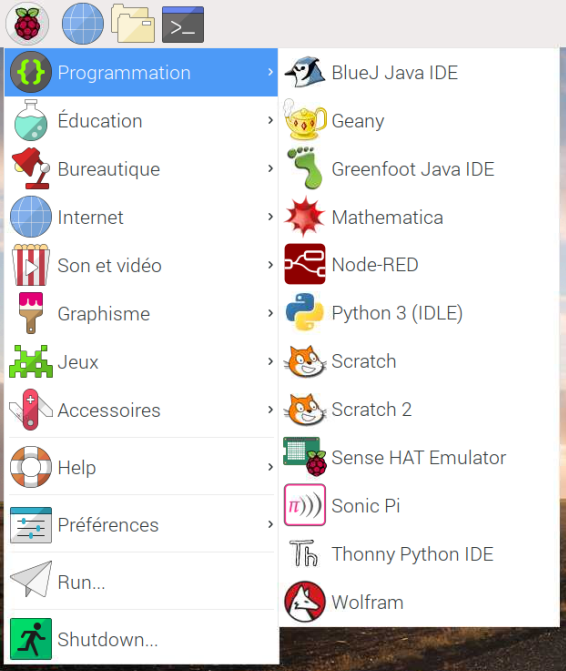
\includegraphics[width=60mm,scale=0.5]{images/raspberry.PNG}
  \caption{Barre de tâche sur raspberry}
  \label{fig:boat1}
\end{figure}

On observe notamment la présence de Scratch et Sonic Pi, logiciels éducatifs dont nous avons déjà parlé et donc pré-installé sur la raspberry. Cela permet de facilement envisager des cursus d'enseignements liés à la raspberry. De plus Sonic Pi possède une fonctionnalité qui le lie à Minecraft \cite{68}, on peut donc plus ou moins lier les idées vu précédemment et créer un enchaînement logique.

\newpage

\section{Synthèse sur l'apport}

Les idées proposées dans l'apport ont un point commun. Partir de quelque chose de connu, que ce soit intriguant ou amusant pour en faire un projet éducatif. Si l'on a un sujet parlant pour les élèves et qui en plus propose de leur apprendre des choses on a alors le ludique et la motivation en un. Par exemple pour le Rubik's Cube en plus de savoir déjà ce qu'est un Rubik's Cube l'élève peut désormais entrevoir comment le résoudre, ce qui est déjà amusant tout en apprenant les algorithmes. Il en est de même pour Minecraft, il y a en effet beaucoup de domaines sous-jacents que l'on peut lier à Minecraft (opérateurs logique, système de client-serveur, lien avec Sonic Pi). De base le principe de Minecraft est lié à la créativité. Nous avons vu d'ailleurs dans l'état de l'art que l'association de la créativité (sujet qui est de base important chez l'enfant) avec l'apprentissage donne de bons résultats. Ces outils nous permettent donc d'aller plus loin que cet existant en proposant en plus de cela un environnement connu.

Malheureusement, la plupart des solutions possèdent des points négatifs, déjà certaines ne sont tout simplement pas implémentables aujourd'hui (cas World Of Warcraft), et d'autres posent le soucis du manque de données quant aux résultats pédagogiques de la méthode. Cependant, étant donné que l'on arrive forcément à lier les idées à des concepts informatiques on peut facilement supposer que cela peut avoir un impact positif. Il faut cependant réfléchir sérieusement à un dispositif d'apprentissage avec ces idées (découper en leçon, quels concepts apprendre et à quel moment, faire un cours récapitulatif sur ce qu'ont appris les élèves etc...).

\newpage